\documentclass{article}
\usepackage{graphicx}
\usepackage[margin=1.5cm]{geometry}
\usepackage{amsmath}

\begin{document}

\title{Wednesday Reading Assessment: Unit 1, Capacitance}
\author{Prof. Jordan C. Hanson}

\maketitle

\section{Memory Bank}

\begin{itemize}
\item $\vec{E}(x) = -\frac{dV}{dx}$ ... E-field from voltage.
\item $C_{tot}^{-1} = C_1^{-1} + C_2^{-1}$ ... Total capacitance of two capacitors in series.
\item $C_{tot} = C_1 + C_2$ ... Total capacitance of two capacitors in parallel.
\end{itemize}

\section{Electric Field}

\begin{enumerate}
\item Suppose a charged system is arranged such that the potential is
\begin{equation}
V(x) = a x ^2 + b x + c
\end{equation}
What is the electric field as a function of $x$? \\ \vspace{0.25cm}
\item What are the units of $a$, $b$, and $c$?
\begin{itemize}
\item A: Volts per meter, volts per meter, and volts
\item B: Volts, volts, and volts
\item C: Volts per meter-squared, volts per meter, and volts
\item D: Volts per meter, volts per meter-squared, and volts
\end{itemize}
\item What is the value of the E-field at $x=1$ m, if $a = 1$, $b = 0.5$ and $c=-1$ (all in the appropriate units)? \\ \vspace{1cm}
\end{enumerate}

\section{Capacitance}

\begin{enumerate}
\item Consider Fig. \ref{fig:caps}.  Suppose each capacitor has a value of 10 $\mu$ F.  (a) What is the total capacitance in circuit (a) and circuit (b)?  (b) What is the total charge stored in each?
\begin{figure}
\centering
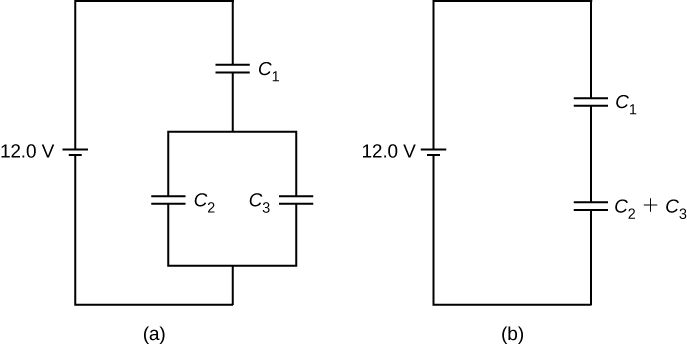
\includegraphics[width=0.4\textwidth]{caps.jpeg}
\caption{\label{fig:caps} Two systems of capacitors.}
\end{figure}
\end{enumerate}

\end{document}
